\noindent 
% \textcolor{blue}{
% The focus of these sections is to source material from Sec.~\ref{sec:apps} and lay out similarities and differences.
% }
Real-time/accelerated AI inference show promises in improving the discovery potential at current and planned scientific instruments across the domains as detailed in Sec.~\ref{sec:apps}. Design of high performant specialty systems for real-time/accelerated AI applications requires particular attention to the figure-of-merit of the target domain's ML algorithm. 
It might be dominated by its latency per inference, computational cost (e.g., power consumption), reliability, security, and ability to operate in extreme environments (e.g., radiation). 
For instance, ML might need to: trigger acquisition systems for rare events with $\sim$100\unit{ns} latency on the Large Hadron Collider~\cite{Duarte:2018ite}; analyze multi-channel ambulatory health monitors at kilohertz frequencies where wireless transfer of data is not possible due to power limitations ($\sim$50 iPhone batteries/day for data transfer) or security requirements; or to keep pace with materials spectroscopy data streams on the order of terabits per second~\cite{Hart2017-bf}.
Furthermore, real-time-analysis of advanced scientific instrumentation must have uninterrupted allocation of computing resources and patient sensitive information processed by wireless health devices must be secured. Such features and characteristics create quantifiable guidelines for understanding distinctions and commonalities among domains and applications. 
Thereby, we can coordinate efforts towards creating fundamental design principles and tools, which may address needs across seemingly disparate domains. 
Appropriate data representation is an essential first step of the design process as it determines the choice of NN architecture to be implemented in real time systems that need to meet the performance targets outlined above. 
Prominent data representations of different scientific instruments are summarized below. 
Other areas of overlap across domains such as NN and hardware co-design tools and workflows, NN complexity reduction with quantization and pruning are also recent technology advancements in real-time/accelerated AI and therefore are outlined in Section~\ref{sec:technolog_sota}.

\subsection{Data representations}
Data representation used in a particular domain influences both the computation system and data storage. One global classification for data representations across domains can be considered as being into raw versus reconstructed data. 
The data representation often varies depending on the stage of the reconstruction and the upstream steps in the data processing pipeline. Existing applications include fully connected NNs that often take pre-processed expert feature variables as inputs or CNNs when the data is of image nature. 
On-going development of domain knowledge inspired NN algorithms could further take advantage of the expert features in the accuracy and efficiency as detailed below.
To fully exploit the power of advanced NNs and bring it closer to data creation for minimum information loss, more suitable representation of the raw data, e.g as point clouds, needs to be employed. 
Prominent representations for raw data from different experimental and measurement systems are:
    \begin{itemize}
        \item \textbf{Spatial Data}: Used for describing physical objects in geometric space. There are two main types, called vector and raster data. 
        Vector data, in turn, can be comprised of points, lines, or polygons. Raster data refers to a grid of pixels, such as images, but pixels can also represent other measurements such as intensity, charge, field strength, etc.
        \item \textbf{Point Clouds}: Can be considered a type of spatial data. 
        This data representation is created by collating a set of spatial data, i.e., points in a 3D space, that usually form an object in space collectively. 
        \item \textbf{Temporal Data}: Used to represent the state of a system/experiment at a particular time. Data collected across time, in a specific order, is classified in this manner. 
        Time-series data is a subset of this representation, where data is sampled at regular time intervals. An example of time-series data can be seen in Fig.~\ref{fig:supernova}, for the specific case of supernova classification.
        \item \textbf{Spatio-Temporal Data}: Measurements and observations of a system can be collected across both the space and time dimensions. 
        In that case, the data can be considered as spatio-temporal. 
        \item \textbf{Multispectral Data}: Used to represent outputs of multiple sensors that capture measurements from multiple bands of the electromagnetic spectrum. Multispectral representation is commonly used in the context of imaging, involving sensors that are sensitive to different wavelengths of light. 
        This usually involves in the order of few to 10s of spectra.    
        \item \textbf{Hyperspectral Data}: Used to represent measurements from a high number of spectra, e.g., in the order of 100s. 
        These images collected from different narrow band spectra are combined into a so called hyperspectral cube with three main dimensions. 
        The first two reference the 2D spatial placement (e.g., earths surface) while the third dimension represents the complete spectrum content at each ``pixel'' location.  
    \end{itemize}  

 \begin{figure*}[tbh!]
     \centering
     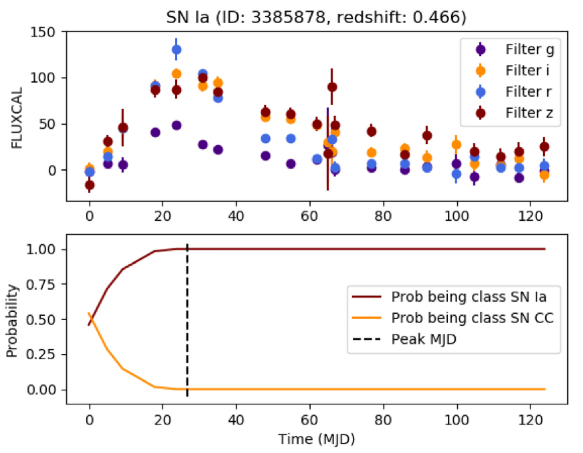
\includegraphics[width = 0.55\textwidth]{figures/supernova_classification.png}
     \caption{Simulated type Ia supernova light-curve and classification. 
     Top: calibrated flux evolution in different DES band-passes as a function of normalized time (the first photometric measurement is set to time equals zero). Bottom: Baseline RNN classification probability evolution with respect of time, no host-galaxy redshift information was provided. 
     At each photometric measurement, classification probability is obtained. Maximum light of the simulated supernova is shown in a gray dashed line and simulated redshift of the supernovae is shown on the top $z = 0.466$. 
     We highlight that redshift is not used for this classification but can improve results. 
     Our Baseline RNN classifies this light-curve as type Ia SN with great accuracy before maximum light, it only requires a handful of photometric epochs. \cite{supernova_2019}.}
     \label{fig:supernova}
 \end{figure*}
 
In Table~\ref{tab:representations}, we match these data representations to scientific application domains and give a brief description.  
We highlight the data representations which are particularly important for a specific domain.  
We will give more detailed examples below.  


Cost of data communication (in terms of latency) and data storage (in terms of the cost of acquiring and managing the physical storage resources) present important challenges. Particularly, application domains, which require real-time analysis and/or real-time feedback demand highly optimized data analytics solutions. 
Applications that rely on hyper-spectral data are faced with an ever increasing rate of data input across the electromagnetic spectrum. High-speed data reduction is required in these domains. 
Applications that generate large scale point clouds similarly demand efficient compression on their spatial data. 
Application domains that handle multi-spectral data with limited spatial resolution require ultra-fast reconstruction in order to enable real-time control feedback. Another challenge is posed by applications that rely on accurate analysis of streaming time-series data, yet they are forced to perform under highly limited storage and communication resources, either due to privacy and security concerns or limitations of the associated edge devices.  

Some current efforts in developing ML solutions to data processing front-ends focus on developing autoencoder based compression engines~\cite{ieee_nss_talk_1_2020, DiGuglielmo:2020eqx}. 
ML-based dimensionality reduction for hyper-spectral data is another direction, which has drawn attention~\cite{Agar2019}. 
Deep learning-based approaches are investigated for image reconstruction; the field of material sciences being one of the most active fields in that regards~\cite{Schmidt_nature2019}. 


\begin{table*}[]
    \centering
    \footnotesize
    \begin{tabular}{|c|c|c|c|c|c|c|}
    \hline
       Domain & Spatial & Point Cloud & Temporal & Spatio- & Multi/Hyper- & Examples\\
              &         &             &          & Temporal & spectral & \\
    \hline
        LHC & \checkmark \checkmark & \checkmark \checkmark & \checkmark & \checkmark & -- & detector reconstruction\\
        Belle-II/Mu2e & \checkmark \checkmark & \checkmark \checkmark & -- & -- & -- & track reconstruction\\
        Material Synthesis & \checkmark & -- & \checkmark & \checkmark \checkmark & \checkmark \checkmark & high-speed plasma imaging \\
        %  &  &  & &  &  & plasma plume\\
        Accelerator Controls & \checkmark & -- & \checkmark \checkmark & -- & -- & beam sensors\\
        Accelerator neutrino & \checkmark \checkmark & \checkmark \checkmark & \checkmark & \checkmark & -- & detector reconstruction \\
        Direct detection DM & \checkmark \checkmark & \checkmark \checkmark & \checkmark & \checkmark & -- & energy signatures \\
        EIC & \checkmark \checkmark & \checkmark \checkmark & \checkmark & \checkmark & -- & detector reconstruction\\
        Gravitational Waves & \checkmark & -- & \checkmark \checkmark & -- & -- & laser inference patterns\\ 
        Biomedical engineering & \checkmark \checkmark & -- & -- & \checkmark \checkmark & -- & cell and tissue images \\  
                            %   &  &  &  &  &  & genomic sequence\\  
        Health Monitoring & \checkmark & -- & \checkmark \checkmark & \checkmark & \checkmark & physiological sensor data\\         
        Cosmology & \checkmark \checkmark & \checkmark \checkmark & \checkmark \checkmark & \checkmark  & \checkmark \checkmark & lensing/radiation maps\\         
        Plasma Physics & \checkmark & -- & \checkmark \checkmark & \checkmark & -- & detector actuator signals\\         
        Wireless networking & -- & -- &  \checkmark \checkmark & -- & -- & electromagnetic spectrum \\ 
    \hline
    \end{tabular}
    \caption{Types of data representations and their relevance for the scientific domains discussed in this paper; \checkmark \checkmark = Particularly important for domain, \checkmark = Relevant for domain}
    \label{tab:representations}
    \normalsize
\end{table*}

%%%%%%
\subsubsection{Expert Feature DNNs}

% A simple approach is to multivariate anlysis is to give as input known expert features
% Positive, more interpretable, more efficient
% Negative, limits the way that we can learn from the data, computational efficiency maybe
% A lot of interest in embedding domain expertise into the nerual network learning process

One straightforward approach to building powerful domain-specific ML algorithms is to start with expert domain features and combine them in a neural network or other multivariate analysis technique.  
This embedded expertise has inherent advantages because the input features are interpretable, and correlations between features can yield insight into a particular task while optimizing performance.  
Furthermore, depending on the computational complexity of the domain features, the computation efficiency of such a machine learning approach can be greater than the direct use of raw features.  
However, the downside is that, by using expert features, we rely entirely on the informativeness of such new features.    

Therefore, there is a lot of interest in automating the process of building informative new features from raw features.  In image classification tasks, for example, a lot of progress has been made in extracting high-level data representations through deep neural networks DNNs~\cite{Goodfellow_2016}. 
In DNNs, layers of neurons above the original input signal are built to ensure that each new layer captures a more abstract representation of the data. Each layer constructs new features by forming nonlinear combinations of the features in the layer below. 
This hierarchical approach to feature construction has been effective in disentangling factors of variation in the data~\cite{Hinton_2006,Bengio_2013,Goodfellow_2016}, and has been useful to construct informative and meaningful representations. 
In astronomical images, for example, a DNN starts with low-level pixel information, gradually capturing at upper layers edges, motifs, and eventually entire objects (e.g., galaxies) to provide a broad view of the Universe~\cite{Sanchez_2018,Huertas_Company_2018}. 
The same applies to other fields of science. For example, detecting particles in large accelerators requires transforming low-level signals into dynamic patterns that can be ascribed to specific particles~\cite{Belayneh_2020}. 
In medical imaging, there is a need to quickly identify abnormal tissue from low-level pixel information by gradually capturing global tissue patterns~\cite{Bychkov_2018}. 
The importance of transforming the initial input data into meaningful abstract representations cannot be overstated: it remains one of the most powerful properties of modern neural network architectures.  

Several challenges exist in the construction of increasingly abstract representations using DNNs. One challenge is to incorporate domain knowledge (e.g., physical constraints) into the neural network model. This is important to address the need for excessive amounts of data when training a DNN, and narrow the gap in representational bias between the model and target concept. Under scarce data but abundant domain expertise, adding domain knowledge can expedite the training process~\cite{Xie_2021}, as well as improving the model generalization performance. Another challenge is to develop tools for model interpretability by explaining the semantics of the representations embedded at each layer~\cite{Chakraborty_2017}. This is challenging due to the distributed representation of information in the network architecture. 

Despite the lack of a formal mechanism to attain a seamless integration between a statistical model and domain knowledge, current approaches point to interesting directions, e.g., using knowledge to add training data or to change the loss function~\cite{Vo_2017}. 
Model interpretability in DNNs has seen an upsurge in research over the past years~\cite{Chakraborty_2017}. 
Commonly, studies look at individual units and their activation patterns to elucidate what is learned across layers of neurons. 


\subsubsection{Frame-based images}
Frame-based images are suitable representation of the experimental data in multiple domains such as neutrino detection with time projection chambers in particle physics. An example of this data representation can be seen in Fig.~\ref{fig:repframe} for an electron deposition in the ProtoDUNE neutrino detector.  
A spatial frame is shown by plotting the time coordinate ``Tick'' and wire position in space. Recent developments in neural network architectures exploit the sparsity of the images to reduce the computation complexity for real-time/accelerated ML applications. Other types of experimental data in HEP and many other domains can also be processed to be represented as frame-based images, although often not without information loss. 
\begin{figure*}[tbh!]
    \centering
    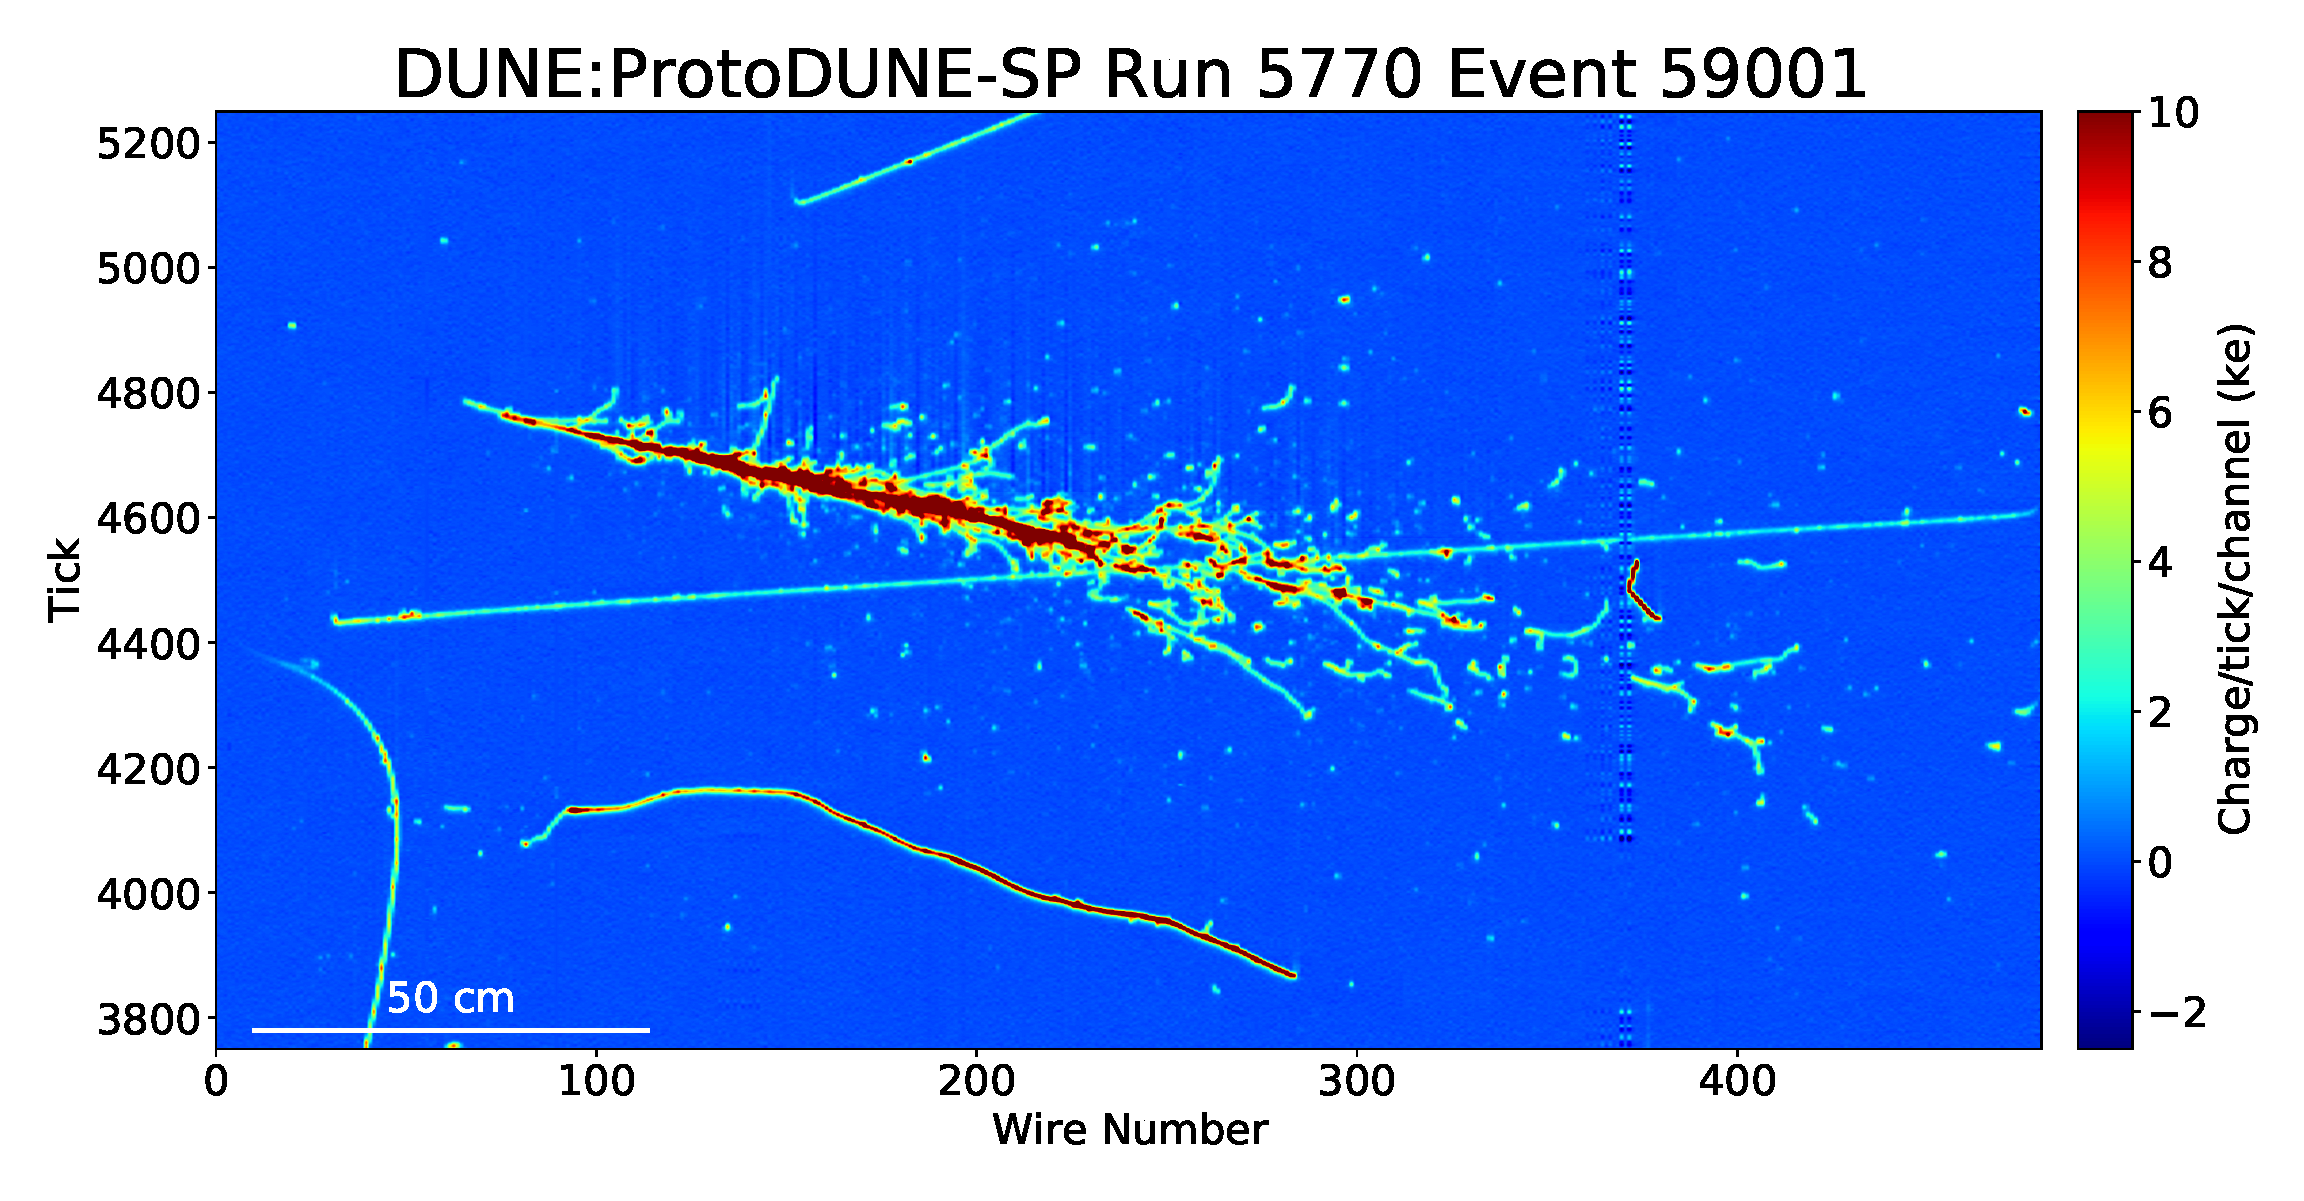
\includegraphics[width = 0.85\textwidth]{figures/R5770_E59001_T1T5T9_w0_480_t3750_5250_sc15.pdf}
    \caption{A 6 GeV/c electron event in the ProtoDUNE detector. The x-axis shows the wire number. The y-axis shows the time tick in the unit of 0.5$\mu s$. The color scale represents the charge deposition.\cite{}}
    \label{fig:repframe}
\end{figure*}

\subsubsection{Point clouds}
 Point cloud data representation is often used in HEP, where multiple frames of event-based measurements collected by a large number of detectors are combined into a data set. Across many HEP applications point clouds commonly help to represent particle jets with data sizes exceeding Pb/s. 
 More broadly, point clouds can be used to capture any 3D space-event and interactions of moving parts in space. 
 A point cloud visualization of the CMS detector at the LHC is shown in Fig.~\ref{fig:repcloud}.  Remnants of proton-proton collisions create sensors signals in a customized and optimized detector geometry and points are illustrated in space. Various types of scan-based imaging data can be represented as point clouds. 
 Other domains such as CT and PET scanning in biomedical engineering and virtual reality also utilize this representation for imaging. 3D scanners used for product design, solid object modeling, architecture, and infrastructure design leverage point clouds as well. Many of these imaging tasks generate point clouds of sizes in the order of several GB to TB. Domains sharing point cloud representation (e.g., HEP and biomedical imaging) also commonly involve spatial characteristics. 
 \begin{figure*}[tbh!]
     \centering
     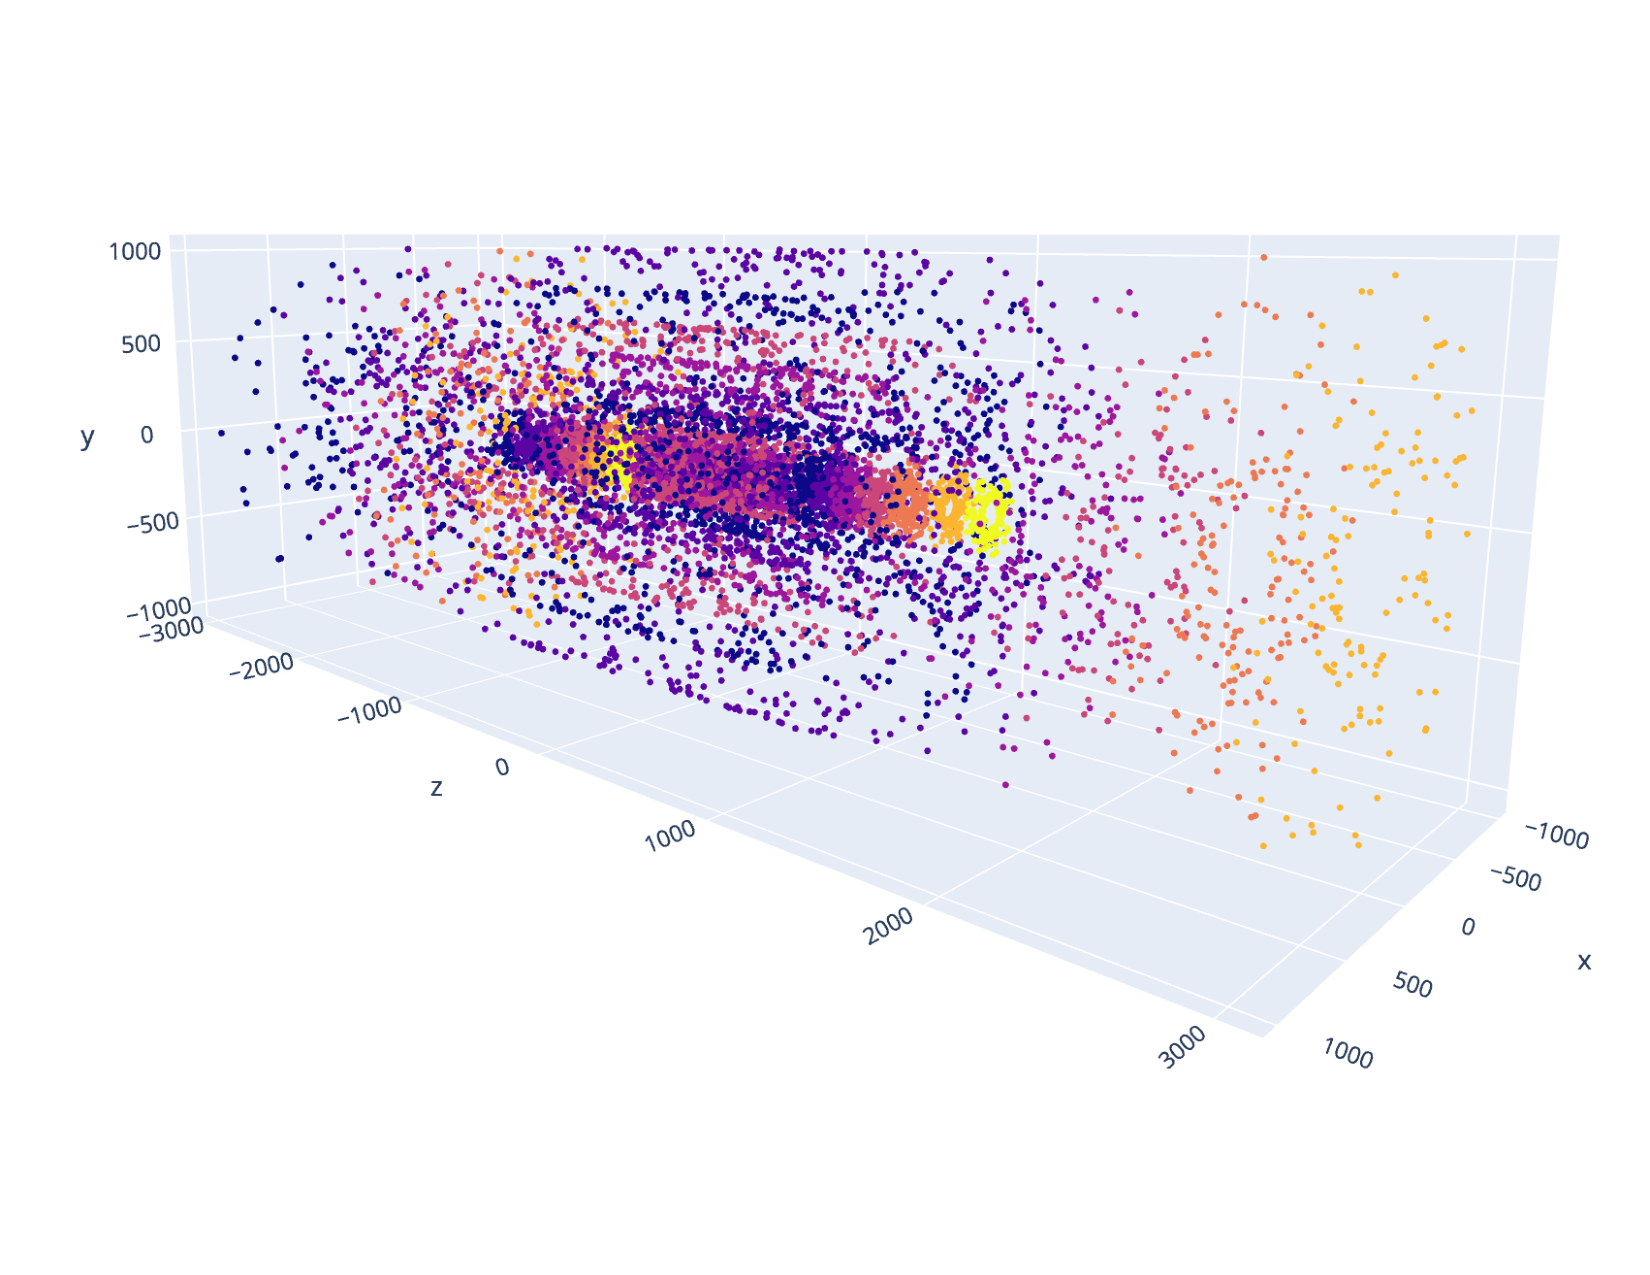
\includegraphics[width=0.85\textwidth]{figures/kaggle-tracking.pdf}
     \caption{Visualization of particle tracking hits in 3D space from the TrackML Kaggle dataset~\cite{cmseventdisplay}}
     \label{fig:repcloud}
 \end{figure*}
 
 \subsubsection{Multi-/Hyperspectral Data}
 Multispectral data is common between wireless health monitoring and wireless communication systems. 
 A set of physiological sensors, often representing different modalities, are combined into a multispectral data set for health monitoring and intervention systems. 
 For wireless communication, signal interference and network traffic conditions are captured via multispectral data. 
 Both domains capture this data across the time domain, so also exhibit temporal features. Furthermore, in both domains generated data size can be considered relatively smaller (ranging from 100s of Mb/s to 10s of Gb/s), compared to the rest of the domains discussed in this article. 
 Hyperspectral data is used across many astronomy applications, medical imaging, and electron microscopy, which is used to drive many materials science design and discovery applications. 
 An example of hyperspectral data in electron microscopy is shown in Fig.~\ref{fig:rephyper}.  
 An electron probe is rastered over a sample under study and diffraction patterns are captured on a pixelated detector.  
 The pixelated detector captures many images as the electron probe is scanned across the sample.  Emerging multimessenger astronomy applications further emphasize the utility of hyperspectral data representations combining observations from a wide array of detectors and telescopes. 
 
 \begin{figure*}[tbh!]
     \centering
     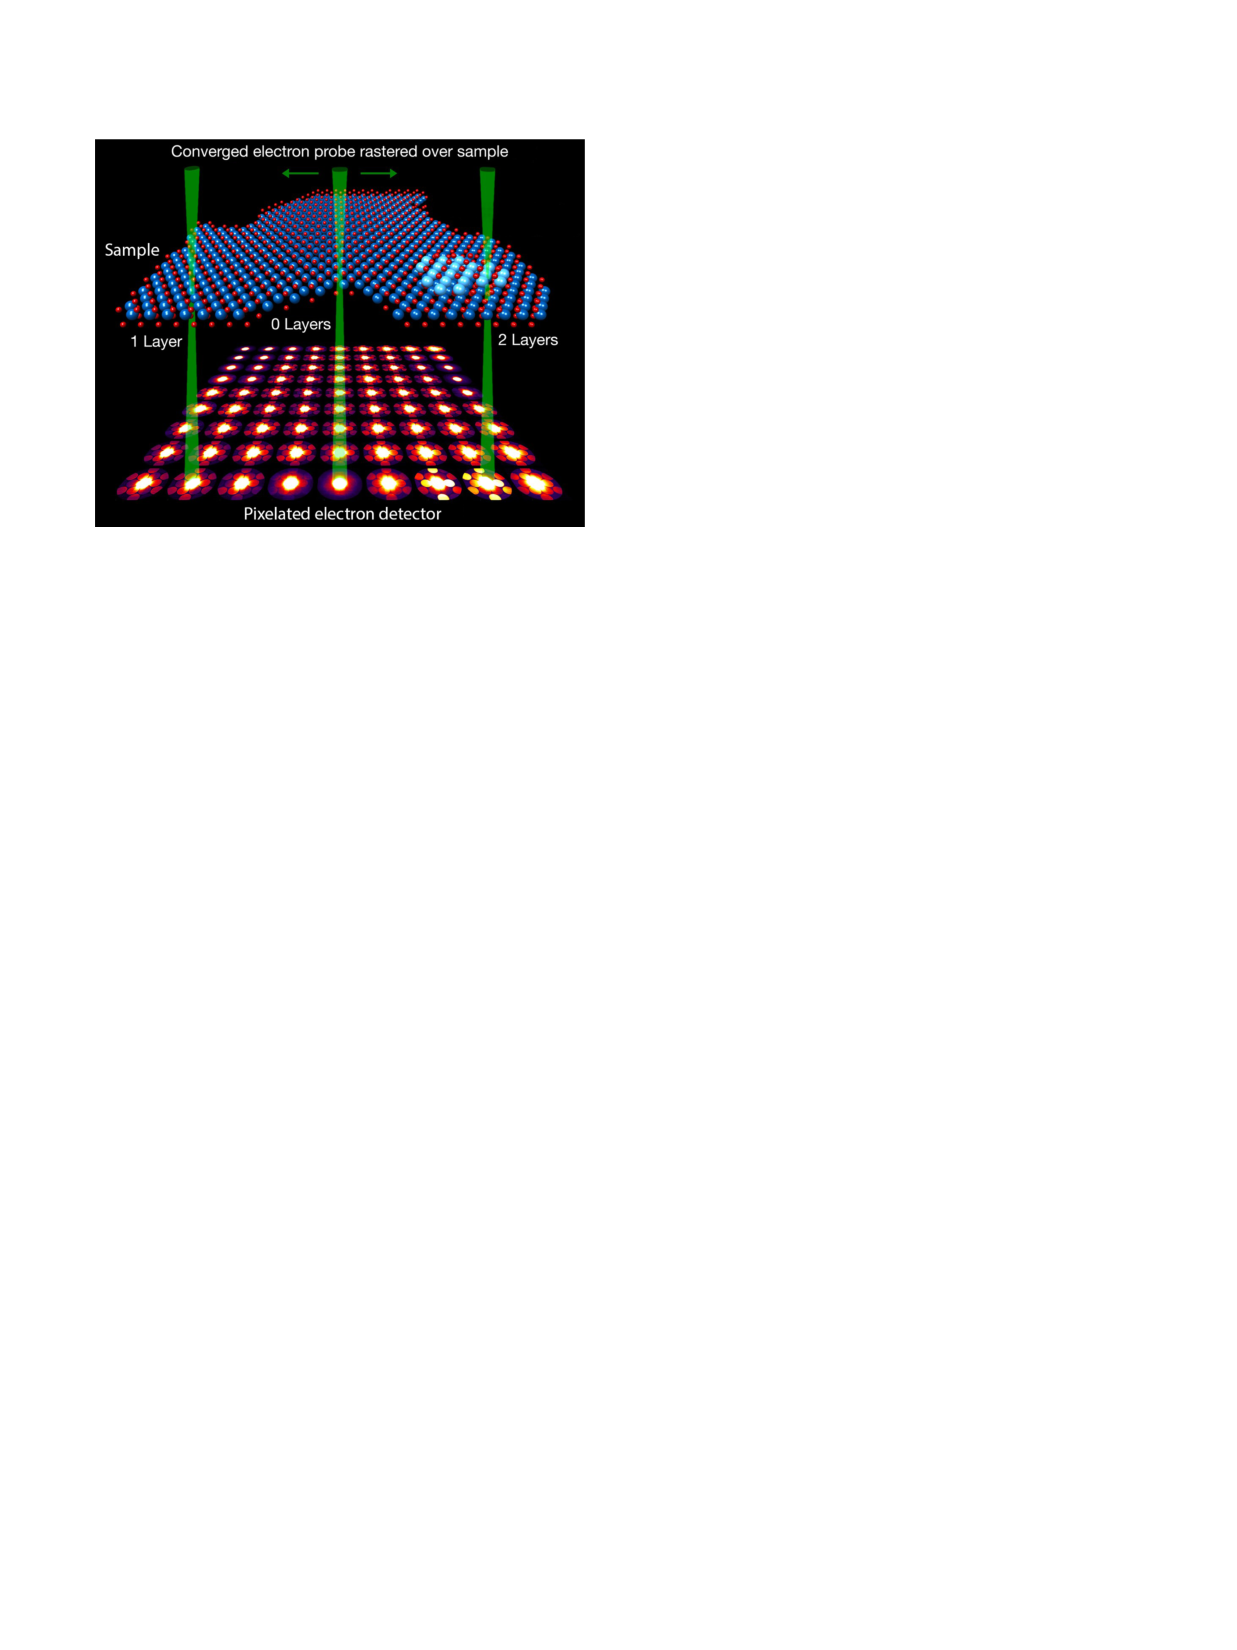
\includegraphics[width = 0.55\textwidth]{figures/TEM.pdf}
     \caption{Experimental 4D-STEM measurement of a dichalcogenide 2D material. Atomic map is inferred from the data, each diffraction pattern represents an average of 7 × 7 experimental images, green STEM probes are labeled for regions of the sample with one layer, vacuum, and two layers \cite{ophus_2019}.}
     \label{fig:rephyper}
 \end{figure*}
 
\subsubsection{Time-series data}
Time-series data is common in experiments that observe dynamically evolving systems in processes such as synthesis for material discoveries or the temporal evolution of the plasma state in nuclear fusion experiments. 
It can be a measurement of high-speed temporally resolved imaging in material science or physics features (density, temperature, current, radiation, fluctuations, etc.) or spatial features of evolving plasma state, as a function of time. 
In-situ diagnostics of the time-series data can either provide alerts to terminate an experiment early that indicates undesired outcome in material science without performing the entire experiment and offline analysis that is time consuming and computationally expensive, thus improves the experiment operation efficiency and accelerates discoveries of material of desired properties. 
This is illustrated in Fig.~\ref{fig:reptime} for accelerator controls at the Fermilab Booster accelerator.  
In this application, magnet voltages which steer proton beams around a synchrotron are recorded at 15~Hz time samples.  
This study builds a digital twin which is used to simulate the Booster data. 
Furthermore, in order to reliably predict and avoid large-scale major disruptions in nuclear fusion experiments, real-time analysis of the time-series data is crucial in guiding the action needed in experimental prediction and control.

 \begin{figure*}[tbh!]
     \centering
     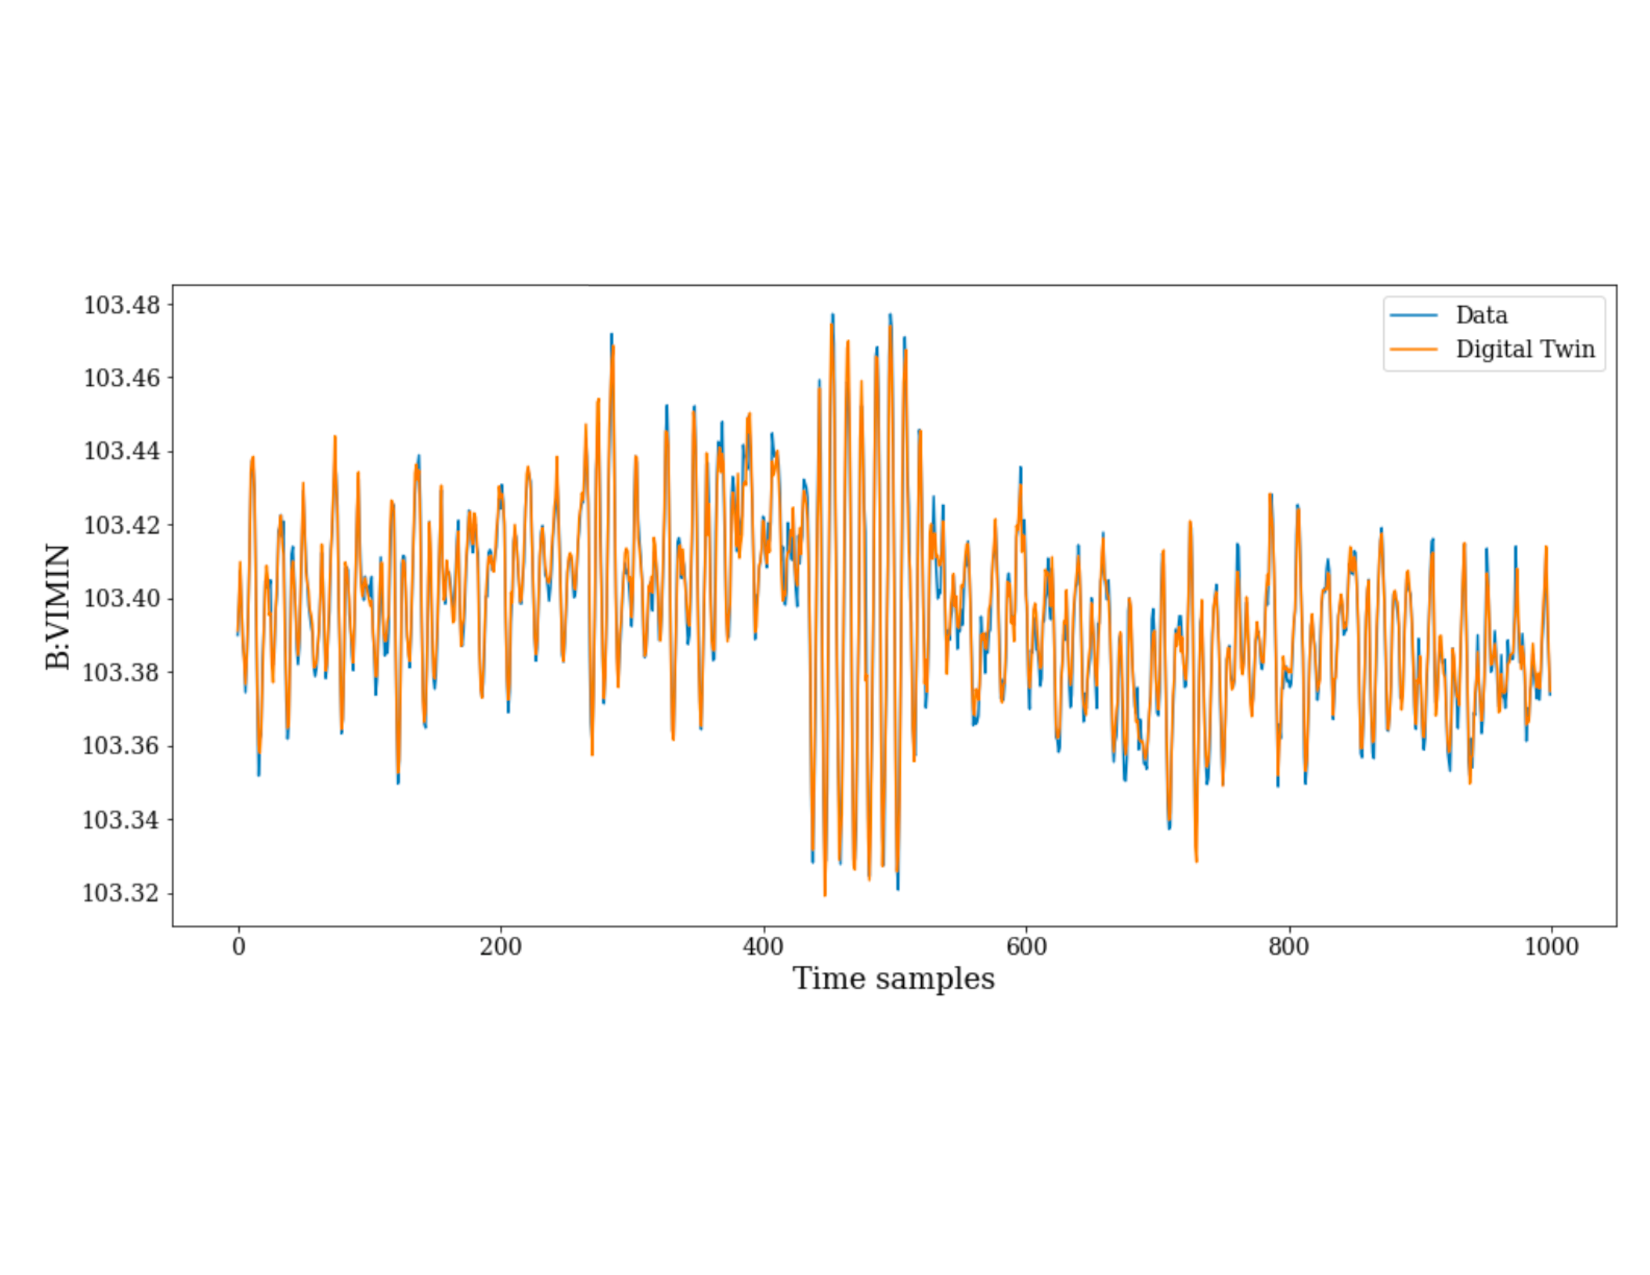
\includegraphics[width = 0.85\textwidth]{figures/Booster.pdf}
     \caption{Selected test data (blue) versus prediction values (orange) from the Booster LSTM surrogate model for the Booster proton synchrotron complex~\cite{John:2020sak}.}
     \label{fig:reptime}
 \end{figure*}
 
\subsection{System constraints}
In this section, we present an overview of desired system properties and constraints that are prevalent across a number of application domains. 
There are unique challenges arising from each scientific application based on sensing technology, the physical processes, and the timescales and data rates and bandwidth.  
These system constraints result in specific choices of data processing platforms, often with multiple compute architectures across the data continuum, such the choice of FPGA-based systems versus embedded processors, GPUs, or custom ASICs. 
Table~\ref{applications} summarizes a number of scientific application domains along with their event rates, system latency constraints and performance requirements, and deployment characteristics. 
We broadly define platforms for integration fast machine learning techniques into ``Soft'', software programmable coprocessors, and ``Custom'', custom embedded computing devices.  Softare programmable systems are often preferred because they are less complex to implement while custom embedded solutions are required when software programmable systems cannot satisfy experimental throughput, bandwidth, or latency constraints.  
We will describe in further detail this distinction below.  
%Table~\ref{data} provides further details and examples of data sources representing each data type. Note that system characteristics that are common to a broad class have been listed first in bold and those that are unique within an individual domain are listed subsequently. 
Examples of these system design choices are the trigger systems for HEP include, LHC reconstruction of collision events, the Belle-II experiment, the Mu2e experiment which deploy custom embedded systems. 
Meanwhile, experiments like the Electron-Ion Collider have data rates which may not require custom hardware solution and could deploy only software programmable solutions for event reconstruction and real-time processing experiments. %although they do not utilize the trigger concept. 
%Another broad category of domains deploy ML solutions to various image processing problems. One of the major distinctions from heavily studied computer vision-based problems is that many of the science applications aim to learn temporal dynamics of a system that is governed by physical processes. 
One final distinction worth discussing concerns the nature of real-time processing and the in-situ versus post-mortem nature of the inference and analysis tasks. 
Examples that we consider in classifying tasks which have different requirements are: data reduction which primarily focuses on limiting data collection rates of experiments for offline analysis; real-time processing and data analysis which is required to extract real-time domain features of the data for tasks like filtering/triggering; and closed-loop controls where data processing provides direct feedback to the operation and continuous control of an experiment. 
These distinctions and their consequences on the computing systems is illustrated in Table~\ref{timing}  

\begin{table*}
\centering
\caption{\label{applications}
Domains and practical constraints: systems are broadly classified as Soft (Software Programmable Computing Devices; CPU, GPU, TPU) and Custom (Custom Embedded Computing Devices: FPGA, ASIC)}
\small
\begin{tabular}{ c c c c c}
\hline
 Domain &  Event Rate & Latency & Systems &  Energy-constrained\\
        % &   Rate &          &         & Constrained\\
 \hline
 \hline
\textbf{Detection and Event Reconstruction} &     &  &         & \textbf{No}  \\ 
LHC/intensity frontier HEP  &  10s Mhz & ns-ms & Soft/Custom        &   \\ 
Nuclear Physics &  10s kHz & ms   & Soft & \\ 
Dark Matter - Neutrino & 10s MHz & us   & Soft/Custom & \\ 
\hline
\textbf{Image Processing}    &         &          &       &   \\ 
Material Synthesis        &  10s kHz   & ms       & Soft/Custom & \\ 
Scanning Probe Microscopy &  kHz   & ms       & Soft/Custom & \\ 
Electron Microscopy       &  MHz   & us       & Soft/Custom & \\ 
Biomedical Engineering   &  kHz   & ms       & Soft/Custom & Yes (mobile settings)\\ 
Cosmology                &            Hz   & s        & Soft           &  \\ 
Astrophysics             &            kHz-MHz   & ms-us  & Soft   & Yes (remote locations)  \\ 
\hline
\textbf{Signal Processing} &           &          &     &     \\ 
Gravitational Waves        &           kHz      & ms      & Soft &  \\ 
Health Monitoring          &  kHz      & ms      & Custom & Yes \\ 
Communications             &  kHz      & ms      & Soft & Yes (mobile settings)\\
\hline
\textbf{Control Systems}   &  &  &   \\ 
Accelerator Controls       &         kHz & ms-us & Soft/Custom  \\ 
Plasma Physics             &         kHz  & ms    & Soft  
\end{tabular}
\normalsize
\end{table*}




%  \begin{table}
%  \caption{Examples of different data representations.}
%  \begin{tabular}{ c c c }
%  \label{data}

%   Domain &  Data Type & Examples \\
%   \hline
%   \hline
%  \textbf{Detection and Event Reconstruction} & Spatial Point Cloud & Detector coordinates in space  \\ 
%                                   & Energy signatures   & Neutral and charged current measurements   \\ 
% \hline
% \textbf{Image Processing}           &  \textbf{Spatial}  &                                \\ 
% Material Synthesis         & Temporal  & high-speed video of plasma plume   \\ 
% Scanning Probe Microscopy  & Temporal   & conductivity, piezoresponse  \\ 
%                           & Hyperspectral time series   & resistivity, magnetic force  \\ 
% Electron Microscopy  & Temporal, Hyperspectral   &  diffraction patterns \\ 
% Biomedical Engineering & Temporal  & cell, tissue images, videos, genomic sequence \\ 
% Cosmology             &  Multispectral  & images, temperature measurements \\ 
% Astrophysics          & Hyperspectral  &  images, electromagnetic spectrum  \\ 
% \hline
% \textbf{Signal Processing}           &    &                                \\ 
% Gravitational Waves         & Spatio-Temporal  & laser interference patterns   \\
% Health Monitoring           & Spatio-Temporal, Multispectral  & physiological sensor data, audio\\
% Communications              & Temporal, Multispectral  &  electromagnetic spectrum  \\
% \hline
% \textbf{Control Systems}   & \textbf{Temporal}  &   \\ 
% Accelerator Controls       &           & sensor readings \\ 
% Plasma Physics             & ??        & ??   \\
% \hline
% \end{tabular}
% \end{table}




\begin{table}
\centering
\caption{\label{timing} Classification of domains and their system requirements with respect to real-time needs.}
\small
\begin{tabular}{ c c c c}
\hline
Domain &  Real-time data reduction & Real-time analysis & Closed-loop Control \\
 \hline
 \hline
\textbf{Detection/Event Reconstruction} &    &                              &   \\ 
LHC                                        & Yes & Yes & No \\ 
Nuclear Physics                            & Yes & No                           & No \\ 
Dark Matter - Neutrino                     & Yes  & No                          & No  \\ 
\hline
\textbf{Image Processing}    &   &              &   \\ 
Material Synthesis        & Yes       & Yes   & Yes \\ 
Scanning Probe Microscopy & Yes       &    &          \\ 
Electron Microscopy       & Yes       &    &      \\ 
Biomedical Engineering   & Yes        &    &      \\ 
Cosmology                & Yes        &  No   & No        \\ 
Astrophysics             & Yes       &  No   & No  \\ 
\hline
\textbf{Signal Processing} &  &          &          \\ 
Gravitational Waves        & Yes         &  No      & No      \\ 
Health Monitoring          & Yes & Yes   & Yes      \\ 
Communications             & Yes & Yes   & Yes      \\
\hline
\textbf{Control Systems}   &     &  &   \\ 
Accelerator Controls       & Yes & Yes & Yes  \\ 
Plasma Physics             & Yes & Yes & Yes      
\end{tabular}
\normalsize
\end{table}

\subsubsection{Software programmable coprocessors}
Historically, first attempts at addressing the computational needs of the problems reviewed in this article have been through software programmable systems. CPU-based local clusters or cloud services as well as cloud computing resources utilizing GPU or TPU-based hardware accelerators are utilized in different applications. One particular concept explored by the HEP community is the GPU as a Service (GPUaaS) model~\cite{krupa2020gpu}. 
This can further be expanded into the Machine Learning as a Service concept, similarly explored within HEP~\cite{kuznetsov2020mlaas4hep}. 
These paradigms involve implementation of machine learning modules to solve a set of physics problems, which are then transferred to GPU or TPU accelerators and accessed by the local CPU ``client'' of the native experimental system. 

One of the major system constraints is the computational capacity, which can be defined in terms of number of floating point operations as far as neural network implementations are concerned. 
Real-time machine learning methods require an ever increasing rate of computational capacity as it directly impacts the \textit{latency per task}. 
The \textit{task} could be a trigger for LHC, reconstruction of an event in accelerator experiments or astrophysics, material synthesis, reconstruction of an image captured by an electron microscope, etc. 
Extreme parallelism would be desired to provide the highest capacity possible to minimize latency and maximize throughput. 
In a processor-based system this can be addressed by increasing the size of the compute cluster. 
Naturally, facility costs impose a limit on the scale of these clusters. 
Another constraint is the available amount of storage coupled with the cost of data movement across the memory hierarchy. 
In the majority of the use cases, the latency involved with moving data from the front-end (detectors, microscopes, sensors, etc.) dominates the total latency. 
One of the prominent performance constraints is related to the utilization and subsequent latency of the network that links the front-end with the back-end. Current limitations on the speed of data movement renders the CPU/GPU cluster-based systems unable to meet the real-time requirements.               
\subsubsection{Custom embedded computing devices}
As the latency and throughput constraints are coupled with challenging practical energy constraints, efforts have been directed towards specialized computing systems to address the hard real-time needs. 
An increasingly attractive paradigm is to design components that are finely optimized for specific steps in the data capture workflow. 
These components can be mapped onto FPGA devices or they can be designed and manufactured as an application-specific integrated circuit (ASIC). 
In the LHC and accelerator domains there is a rich set of FPGA-based demonstrations of front-end data processing systems, which meet microsecond latencies. 
These systems are in charge of tasks such as triggering, event reconstruction, and anomaly detection. Direct and naive implementations of neural networks to perform inference for these tasks can fail to meet the latency requirements, since they often incur significant resource utilization. 
Highest achievable FPGA clock frequency and inference latency is correlated with the resource utilization and percentage occupancy of the device. 
Co-design techniques developed for these applications particularly specialize in extreme quantization and pruning (with an awareness of accuracy) so that resource requirements can be controlled aggressively to ensure inference latency targets. 
These optimizations push the resource usage envelop as far as down as 10s of percent of the FPGA device in order to meet the system constraints and yet demonstrate implementations with high inference accuracy.

Some other applications (e.g., accelerator controls, biomedical and health applications) impose less stringent latency expectations, in the order of ms, where the urgency for resource minimization is alleviated. 
Hence, the focus of the system design can shift from extreme resource economy to enhanced sophistication in the algorithms that are being mapped to the device. 
Inference models can now include deep(er) learning models coupled with advanced video and signal processing engines, as well as local privacy preserving processing tasks (applicable particularly to mobile health and networking and communication applications). 

For mobile and IoT-based deployment of the edge devices resource efficiency emerges as an important factor as it impacts energy consumption.
However, in these applications, energy efficiency can also be achieved by alternative means. 
One option would be selective powering, i.e., creating a resource-rich full featured baseline implementation, which still comfortably meets latency constraints if energy was not an issue, and introducing power gating or standby features to modulate energy consumption during periods of low/no activity. 

There are system constraints, which point the designers to a custom ASIC solution in addition to or in place of FPGA devices. ASICs can address extreme form factor considerations, integration of computation with sensing (e.g., smart photon detectors) into compact front-end devices, tight integration with other mixed signal or analog functionalities, radiation hardening requirements, and ultra-low energy budgets.   
